% fancytikzposter.tex, version 2.1
% Original template created by Elena Botoeva [botoeva@inf.unibz.it], June 2012
% 
% This file is distributed under the Creative Commons Attribution-NonCommercial 2.0
% Generic (CC BY-NC 2.0) license
% http://creativecommons.org/licenses/by-nc/2.0/ 


\documentclass[a1,portrait]{a0poster}

\usepackage{fancytikzposter} 

\usepackage[utf8]{inputenc}
\usepackage{hyphsubst}
%\HyphSubstIfExists{ngerman-x-latest}{
%  \HyphSubstLet{ngerman}{ngerman-x-latest}}{}
%\HyphSubstIfExists{german-x-latest}{
%  \HyphSubstLet{german}{german-x-latest}}{}
\usepackage{zi4}
\usepackage{amsmath} %for matrices
\usepackage{amssymb} %for element of N / R etc
\usepackage{amsthm} % proof
\usepackage[english]{babel} % Beweis etc
\newcounter{theorems}
\usepackage{natbib} % cites
\usepackage{hyperref}

%\usepackage{mdframed}
\usepackage{enumerate}
%\usepackage[hyphenbreaks]{breakurl}

\usepackage{graphicx} %\includegraphics
\usepackage{tikz}
\usetikzlibrary{positioning,fit,patterns}
\usetikzlibrary{shapes}
\usetikzlibrary{arrows}
\usetikzlibrary{arrows.meta}
\usetikzlibrary{positioning,automata} 
\usepackage[all]{xy}
\usepackage{float}
\usepackage{color}
\usepackage{soul} %ul etc
\definecolor{darkgreen}{rgb}{0.0,0.5,0.0}
\definecolor{darkred}{rgb}{0.5,0.0,0.0}
\definecolor{darkyellow}{rgb}{0.5,0.5,0.0}
\definecolor{lightgreen}{rgb}{0.5,1,0.5}
\definecolor{lightgreen2}{rgb}{0.7,0.9,0.7}

\newcommand{\cfbox}[2]{%
    \colorlet{currentcolor}{.}%
    {\color{#1}%
    \fbox{\color{currentcolor}#2}}%
}

\usepackage{listings}
\usepackage{nth}
%\lstset{numbers=left,language=C,frame=lines,commentstyle=\color{darkgreen}\ttfamily,keywordstyle=\color{blue},mathescape,basicstyle=\ttfamily\scriptsize}

\newtheorem{ex}{Example}
\newtheorem*{ex*}{Example}
\newtheorem*{exS}{Example \cite{thwart}}

\newcommand{\matone}{TODO1}
\newcommand{\mattwo}{TODO2}
\newcommand{\mts}{MTS420cc }
\title{\textbf{Anti Bicycle Theft}\bigskip\\Documentation}
\author{Kevin Freeman (\matone)\\ Martin Schwarzmaier (\mattwo)\\Georg-August-Universität Göttingen}
\date{\today}

%%%%% --------- Change here if you want ---------- %%%%%
%% margin for the geometry package, must be changed before using the geometry package
%% default value is 4cm
% \setmargin{4}

%% the space between the blocks
%% default value is 2cm
% \setblockspacing{2}

%% the height of the title stripe in block nodes, decrease it to save space
%% default value is 3cm
% \setblocktitleheight{3}

%% the number of columns in the poster, possible values 2,3
%% default value is 2
% \setcolumnnumber{3}

%% the space between two or more groups of authors from different institutions
%% used in \maketitle
% \setinstituteshift{10}

%% which template to use
%% N1 simple, standard look, with a colored background and gray boxes
%% N2 board with nodes
%% N3 another standard look
%% N4 envelope-like look
%% N5 with a wave-like head, original idea taken from
%%%% http://fc09.deviantart.net/fs71/f/2010/322/1/1/scientific_poster_by_nabuy-d333ria.jpg
%\usetemplate{6}

%% components of the templates
%% (the maximal possible numbers are mentioned as the parameters)
% \usecolortemplate{4}
% \usebackgroundtemplate{5}
% \usetitletemplate{2}
% \useblocknodetemplate{5}
% \useplainblocktemplate{4}
% \useinnerblocktemplate{2}


%% the height of the head drawing on top 
%% applicable to templates N3, 4 and 5
% \setheaddrawingheight{14}


%% change the basic colors
%\definecolor{myblue}{HTML}{008888} 
%\setfirstcolor{myblue}% default 116699
%\setsecondcolor{gray!80!}% default CCCCCC
%\setthirdcolor{red!80!black}% default 991111

%% change the more specific colors
% \setbackgrounddarkcolor{colorone!70!black}
% \setbackgroundlightcolor{colorone!70!}
% \settitletextcolor{textcolor}
% \settitlefillcolor{white}
% \settitledrawcolor{colortwo}
% \setblocktextcolor{textcolor}
% \setblockfillcolor{white}
% \setblocktitletextcolor{colorone}
% \setblocktitlefillcolor{colortwo} %the color of the border
% \setplainblocktextcolor{textcolor}
% \setplainblockfillcolor{colorthree!40!}
% \setplainblocktitletextcolor{textcolor}
% \setplainblocktitlefillcolor{colorthree!60!}
% \setinnerblocktextcolor{textcolor}
% \setinnerblockfillcolor{white}
% \setinnerblocktitletextcolor{white}
% \setinnerblocktitlefillcolor{colorthree}




%%% size of the document and the margins
%% A0
% \usepackage[margin=\margin cm, paperwidth=118.9cm, paperheight=84.1cm]{geometry} 
\usepackage[margin=\margin cm, paperwidth=84.1cm, paperheight=118.9cm]{geometry}
%% B1
% \usepackage[margin=\margin cm, paperwidth=70cm, paperheight=100cm]{geometry}



%% changing the fonts
\usepackage{cmbright}
%\usepackage[default]{cantarell}
%\usepackage{avant}
%\usepackage[math]{iwona}
\usepackage[math]{kurier}
\usepackage[T1]{fontenc}


%% add your packages here
\usepackage{hyperref}





\title{Anti Bicycle Theft}
\author{Kevin Freeman, Martin Schwarzmaier\\
  Practical Course on Wireless Sensor Networks\\
  \texttt{Advised by: Dr. Omar Alfandi \& Arne Bochem, M.Sc.}
}


\begin{document}

%%%%% ---------- the background picture ---------- %%%%%
%% to change it modify the macro \BackgroundPicture
\renewcommand\BackgroundPicture{%
  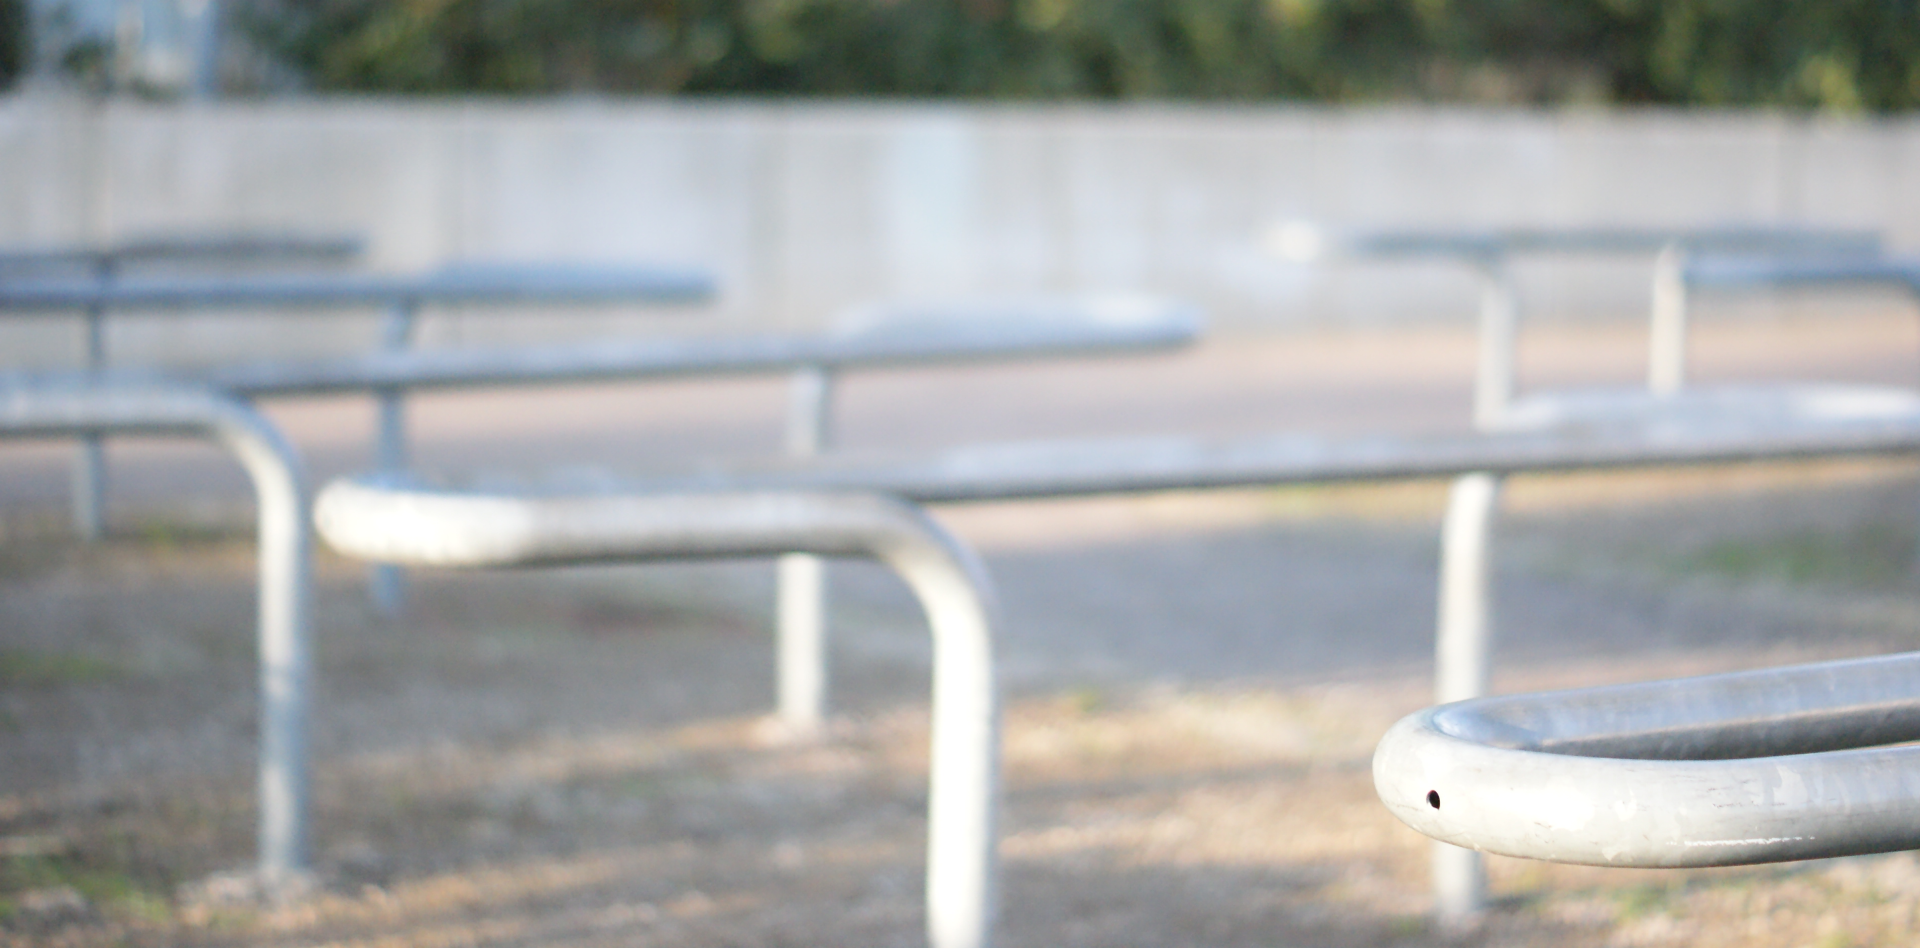
\includegraphics[scale=4]{flatRack.png}}
\ClearShipoutPicture
\AddToShipoutPicture{\BackgroundPicture}

\noindent % to have the picture right in the center
\begin{tikzpicture}
  \initializesizeandshifts
  % \setxshift{15}
  % \setyshift{2}


  %% the title block, #1 - shift, the default value is (0,0), #2 - width, #3 - scale
  %% the alias of the title block is `title', so we can refer to its boundaries later
  \ifthenelse{\equal{\template}{1}}{ 
    \titleblock{47}{1}
  }{
    \titleblock{47}{1.5}
  }

  %% a logo can be added to the title block
  %% #1 - anchor relative to the title block, #2 - shift, #3 - width, #3 - file name
  % \ifthenelse{\equal{\template}{2}}{ 
  %   \addlogo[south west]{(2,0)}{6cm}{unibz_b.png}
  % }{
  %   \addlogo[south west]{(2,0)}{6cm}{unibz_w.png}
  % }


  %% a block node, with the specified position (optional), title and the content
  %% #1 - where (optional), #2 - title, #3 - text
  %%%%%%%%%% ------------------------------------------ %%%%%%%%%%
  \blocknode%
  {Introduction}%
  {
Bicycle theft is a major problem in many cities, especially university towns.
Our aim was to create a system that enables a bike owner to track a stolen bike. While other systems already on the market are trying to accomplish this by using GSM modules we tried to use a minimalistic approach:\\
A tracking GPS module that can be turned on after a bike has been stolen, tracks positions and retransmits them to the user via a short distance wireless interface and represents them on an easy-to-use web interface.\\
\begin{center}
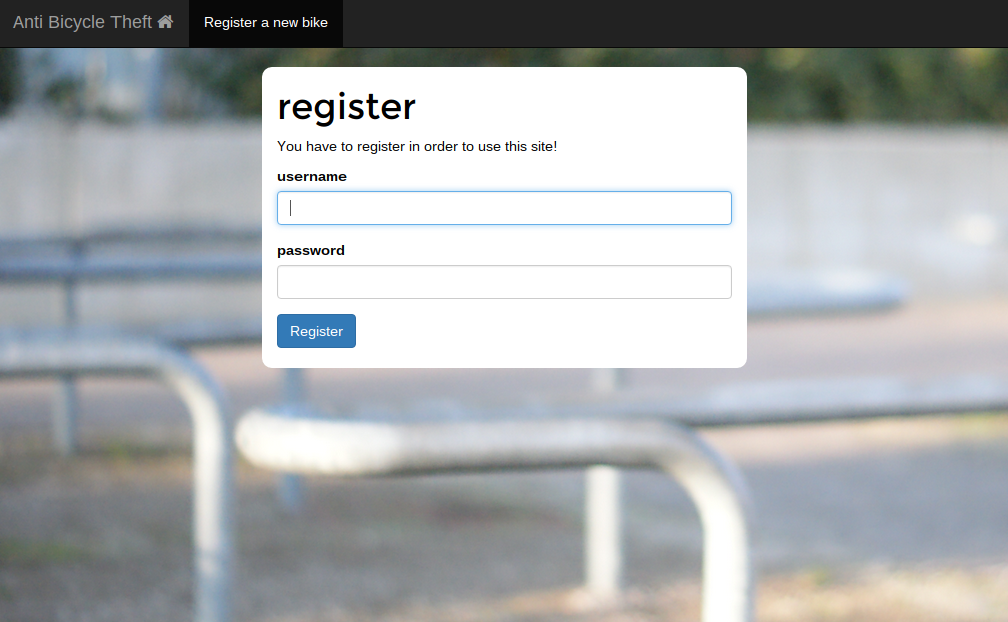
\includegraphics[scale=0.85]{../../project_doc/pics/reg.png}  
\end{center}\vspace{1cm}
  
  %Start with the following document:
%
 %   \coloredbox{colorthree!50!}{
  %    ...
   % }
  }


  %% a callout block
  %% #1 - rotate angle (optional), #2 - from, #3 - where, #4 - width, #5 - text
  %%%%%%%%%% ------------------------------------------ %%%%%%%%%%
  %\calloutblock{($(box.center)+(-2,-8)$)}
  %{($(box.center)+(10,-1)$)}
  %{19cm}
  %{\small
  %  Macro for creating a block node:
  %  \begin{itemize}
  %  \item[] \textbackslash blocknode\{Block Title\}\{Block Content\}
  %  \end{itemize}
  %  Macro \textbackslash blocknode has three parameters. The first one is
  %  optional and it is the position of the block. The first block will be
  %  automatically placed to (\$(firstrow)-(xshift)-(yshift)\$), which is the
  %  left corner below the title block. In most of the templates, (firstrow) is
  %  set to (title.south), where \emph{title} is the alias for the title
  %  block. Each subsequent block is automatically placed to
  %  [(\$(box.south)-(yshift)\$)], i.e., below the previous block aliased
  %  \emph{box}.  You can also use an explicit parameter, e.g., $(-10,30)$ (note
  %  that (0,0) is the center of the poster). The second parameter is the title
  %  of the block. Finally, the last parameter is the  actual content. 
  %}




  %% by default, the position of the new block node is right below the previous
  %% block node, stored in (currenty)
  %% box is the alias of the previous block, so we can refer to its boundaries

  %%%%%%%%%% ------------------------------------------ %%%%%%%%%%
  \blocknode{Used Software}%
  {
\begin{enumerate}
\item Linux with TinyOS
\item NodeJS with Express
\item MongoDB
\item TinyOS Protocols (Dissemination \& Collection \cite{colldiss})
\end{enumerate}
  
  }
  
  %%%%%%%%%% ------------------------------------------ %%%%%%%%%%
  \blocknode{Used Hardware}%
  {
\begin{enumerate}
\item Webserver with TinyOS, e.g. Raspberry Pi
\item IRIS motes
\item USB gateway (connected to the server)
\item MTS420cc sensorboard including GPS antenna
\end{enumerate}\vspace{0.2cm}

\begin{center}
(pictures according to previous enumeration numbered from left to right)\\\vspace{0.55cm}
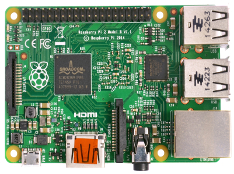
\includegraphics[scale=4.15]{../../project_doc/pics/rasp.jpg}
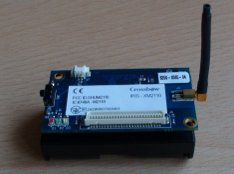
\includegraphics[scale=1]{../../project_doc/pics/mote.jpg}  
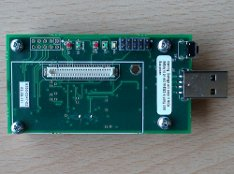
\includegraphics[scale=1]{../../project_doc/pics/gateway.jpg}
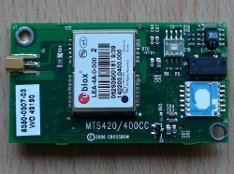
\includegraphics[scale=1]{../../project_doc/pics/420cc.jpg}
\end{center}
  
  
  }
  
  %%%%%%%%%% ------------------------------------------ %%%%%%%%%%
  \blocknode{System Description}%
  {

The system consists of a computer running a webserver, an IRIS mote connected to the it via USB, a set of relay IRIS motes and so called bicycle IRIS motes. The process begins after a user marked his bike as stolen using the system's webapplication using an \texttt{ID}. The webserver will relay this \texttt{ID} to the basestation which broadcasts it to all relay motes via dissemination\cite{colldiss}. When a bike passes a relay mote it establishes a connection and checks whether its \texttt{ID} is being disseminated. If this is the case the bicycle mote will turn on its GPS module and start recording its position in combination with a timestamp.\\
The next time the bike passes a relay mote the position data is transfered, collected\cite{colldiss} at the base station and made available to the user on the webapplication.

\vspace{0.5cm}
\begin{center}
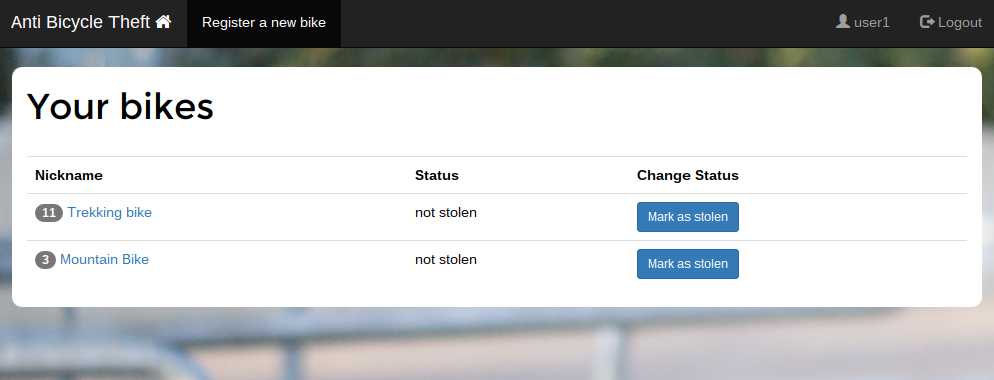
\includegraphics[scale=0.94]{../../project_doc/pics/mark.png}  
\end{center}
  
  
  }
  

  


  %%%%%%%%%%%%% NEW COLUMN %%%%%%%%%%%%%%% 
  \startsecondcolumn 
  
  
  %%%%%%%%%% ------------------------------------------ %%%%%%%%%%
  \blocknode{Topology}%
  {

\begin{center}

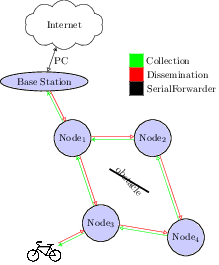
\includegraphics[scale=0.85]{../../project_doc/standalone_topology/topo.png}
\end{center}
%\caption{Example network including protocols used}\label{fig:topo}

  
  }  
  %%%%%%%%%% ------------------------------------------ %%%%%%%%%%
  \blocknode{Conclusion}%
  {
The system we proposed an implemented prototypically allows a user to remotely turn on a location tracking device, collect data over extended periods of time. This works even if his bike is not in range of a network after it has been activated. Using an easy-to-use webinterface bicycles are able to be quickly reported as stolen. Gathered location data can be conveniently displayed on a digital map.\\

\begin{center}
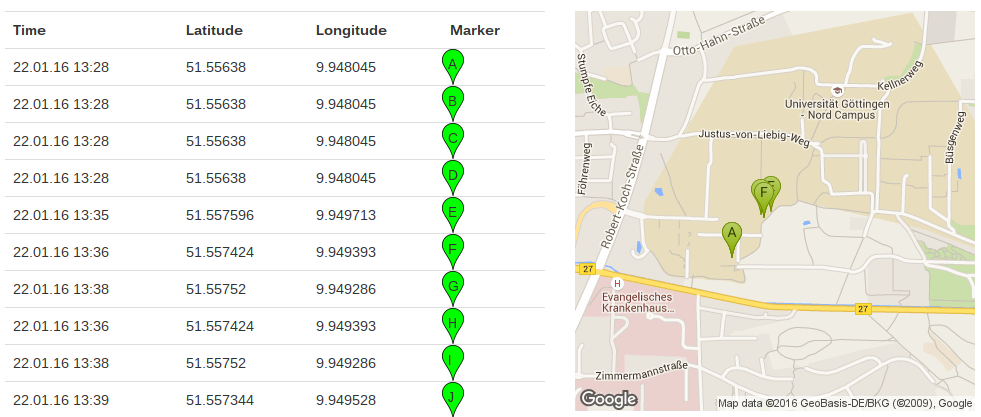
\includegraphics[scale=0.94]{../../project_doc/pics/concl.png}  
\end{center}


Future work is needed to determine how battery usage can be minimized (e.g. by replacing GPS with WiFi positioning) and whether a sufficient relay network can be established at reasonable costs.  
  
  
  }
  


  
  %%%%%%%%%% ------------------------------------------ %%%%%%%%%%
  \blocknode{References}%
  {
\renewcommand\refname{}\vspace{-1cm}
\nocite{bka}
\nocite{colldiss}
\nocite{golembike}
\nocite{leash}
\bibliographystyle{plain}
\bibliography{src}{}  
  
  }


  %%%%%%%%%% ------------------------------------------ %%%%%%%%%%
  %\calloutblock{($(box.south east)-(8,-2)$)}
  %{($(box.south east)-(16,2)$)}
  %{30cm}
  %{
  %  There are also callout blocks that allow for a more interesting layout of the
  %  poster. 
  %  \begin{itemize}
  %  \item[] \textbackslash calloutblock[rotate angle]\{from
  %    coordinate\}\{coordinate\}\{Block Width\}\{Block Content\} 
  %  \end{itemize}
  %  The alias for such blocks is \emph{note}.
  %}


  %% to place the next node centered vertically in the second column, we can
  %% obtain the y-coordinate of the previous node using macro
  %% \getcurrentrow{note}, where note is the alias of the callout node, and
  %% then specify the coordinate of the next node using coordinate (currentrow)
  %\getcurrentrow{note}


  %% a plain block
  %% #1 - rotate angle (optional), #2 - where, #3 - width, #4 - title, #5 - text
  %%%%%%%%%% ------------------------------------------ %%%%%%%%%%
  %\plainblock{($(currentrow)+(xshift)-(yshift)$)}%[($(currenty)+(0,10)$)]%
  %{32}{Plain blocks} %
  %{These blocks are similar to callout blocks. They allow for specifying the
  %  title of the block.
  %  \begin{itemize}
  %  \item[] \textbackslash plainblock[rotate angle]\{coordinate\}\{Block Width\}\{Block
  %    Title\}\{Block Content\} 
  %  \end{itemize}
  %}


 
  %% the coordinate (currenty) is used in the default placing of the next blocknode
% \getcurrentrow{note}
 %\coordinate (currenty) at ($(currentrow)+(xshift)-(yshift)$);



   %%%%%%%%%%%%% NEW COLUMN %%%%%%%%%%%%%%% 
  %% (if column number is 3)
  \startthirdcolumn

  %%%%%%%%%% ------------------------------------------ %%%%%%%%%%
  



\end{tikzpicture}


\end{document}




